\documentclass{beamer}
\usepackage[english]{layout}
\usepackage[utf8]{inputenc}
\usepackage[english]{babel}
\usepackage[T1]{fontenc}
\usepackage{amsmath, soul, color, multicol, type1cm, verbatim, latexsym, dsfont, float, listings}
\usepackage[official]{eurosym}
\usepackage{beamerthemesplit}
\usetheme{Frankfurt}
\usecolortheme{lily}
%\usefonttheme{structuresmallcapsserif}
\usefonttheme{professionalfonts}
\setbeamercovered{transparent}

%NeSI Colors <---------------------------------------------------------------------------------------
\usecolortheme[RGB={47, 68, 71}]{structure} 
\definecolor{nesidark}{HTML}{2F4447}
\definecolor{nesilight}{HTML}{CED9DF}
\definecolor{nesigrey}{gray}{0.7}
\definecolor{nesilightgrey}{gray}{0.98}
\definecolor{nesidarkgrey}{gray}{0.3}
\definecolor{nesiblue}{HTML}{2B9FC2}
\setbeamercolor{block title}{fg=black,bg=nesigrey}
\setbeamercolor{block body}{bg=nesilightgrey,fg=nesidarkgrey}
\setbeamercolor{block body alerted}{bg=white,fg=black}
\setbeamercolor{alerted text}{bg=white,fg=black}

\setbeameroption{show notes}

\setbeamerfont{title}{size=\huge}
\frenchspacing
\hyphenation{NeSI}

\newenvironment{topcolumns}{\begin{columns}[t]}{\end{columns}}
\newcommand\BackgroundPicture[1]{%
\setbeamertemplate{background}{%
\parbox[c][\paperheight]{\paperwidth}{%
\vfill \hfill \includegraphics[height=0.9\paperheight]{#1}
\hfill \vfill
}}}

\setbeamertemplate{blocks}[default]%[shadow=false]
\useinnertheme{circles}
\setbeamertemplate{title page}[default][center,rounded=false,shadow=false]
%\setbeamertemplate{title page}[default][center, wd=60mm, colsep=-4bp,rounded=true]

% Fancy Footer Content    <-----------------------------------------------------------------------------
%\setbeamertemplate{footline}{
%   \unilogo
%   \dsglogo
%   \begin{beamercolorbox}[ht=4ex,leftskip=1.4cm,rightskip=.3cm]{author in head/foot}
%    \usebeamercolor{nesiblue}
%    \hrule
%    \vspace{0.1cm}
%    \insertdate \hfill \inserttitle \newline
%    \insertshortauthor \ - \insertshortinstitute \hfill \insertframenumber
%   \end{beamercolorbox}
%   \vspace*{0.1cm}
%} 
% Reference http://joerglenhard.wordpress.com/2011/08/04/beamer-customization-ii-footline-with-multiple-lines/
% http://joerglenhard.wordpress.com/tag/beamer/
% https://github.com/lenhard/ub-beamer


\title{Using NeSI HPC Resources}
%\subtitle{Computational Science team}
\author{NeSI Computational Science Team \\(support@nesi.org.nz)}
\date{}


\begin{document}

{
\setbeamertemplate{background canvas}{
\includegraphics[height=0.99\paperheight]{NeSI_img/Slide00.png}} 
\begin{frame}[plain]
\vspace{1cm}
\titlepage
\end{frame}
}


%\BackgroundPicture{NeSI_img/SlideXX.png}
\begin{frame}
\frametitle{Outline}
\begin{multicols}{2}
   \tableofcontents
 \end{multicols}
 \end{frame}


%%%%%%%%%%%%%%%%%%%%%%%%%%%%%%%%%%%%%%%%%%%%%%%%%%%%%%%%%%%%%%%%%%%%%%%%%%%%%%%%%%%%%%%%%%%%%%%
%%%%%%%%%%%%%%%%%%%%%%%%%%%%%%%%%%%%%%%%%%%%%%%%%%%%%%%%%%%%%%%%%%%%%%%%%%%%%%%%%%%%%%%%%%%%%%%

\section{About Us}
\subsection{About NeSI}
\frame[t]
{
  \frametitle{About Us}
\begin{center}
\vspace*{1cm}
 
\includegraphics[width=225pt]{NeSI_img/nesi_logo.jpg}\\
 
\includegraphics[width=50pt]{NeSI_img/logo-u-of-a.jpg}
 
\includegraphics[width=50pt]{NeSI_img/logo-u-of-c.jpg}
 
\includegraphics[width=50pt]{NeSI_img/logo-niwa.jpg}
 
\includegraphics[width=50pt]{NeSI_img/logo-ministry-of-si.jpg} 
 
\includegraphics[width=50pt]{NeSI_img/logo-manaaki-whenua.jpg}
 
\includegraphics[width=50pt]{NeSI_img/logo-u-of-o.jpg}
\end{center}
}

\frame[t]
{
  \frametitle{About Us}
      \begin{block}{Support}
   \begin{itemize}%[<+-| alert@+>]
	\item Email \url{support@nesi.org.nz}
	\item Creates a support ‘ticket’ where we can track the history of your request
	\item You can also arrange to meet us to discuss any issues
   \end{itemize}
   \begin{center}
   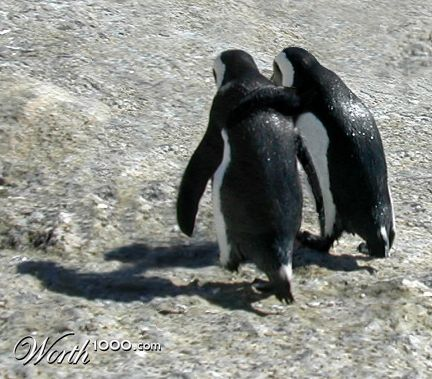
\includegraphics[width=100pt]{NeSI_img/pingu-friend.jpg}
   \end{center}
  \end{block}
}

\subsection{Our Facilities}
\frame[t]
{
  \frametitle{Our Facilities}
      \begin{block}{NeSI Facilities}
   \begin{itemize}%[<+-| alert@+>]
	\item NeSI provides several kind of HPC architectures and solutions to cater for various needs.
     \begin{itemize}
     	\item Bluegene/P
	    \item Power6 and Power7
   		\item Intel Westmere
		\item Intel SandyBridge
		\item Kepler and Fermi GPU servers
		\item Intel Xeon Phi Co-Processor
   \end{itemize}
	\item Supported applications can run on across several NeSI architectures.% but for some of them there are more suitable architecture.
	\item We can install and study the scalability in all the NeSI resources and find the most suitable environment for your case.
	\item See NeSI website for facility specs and application details.
   \end{itemize}
  \end{block}
}

\frame[t]
{
  \frametitle{Our Facilities}
      \begin{block}{BlueFern Supercomputing Center}
   \begin{itemize}%[<+-| alert@+>]
	\item Funded by the \textbf{BlueFern, University of Canterbury} with co-investment from the NZ Government through \textbf{NeSI}.
	\item Currently have 8612 CPU cores across 2061 hosts.
	\item About 9.6 TB of memory and 71.4 TFLOPS (distributed).
	\item Shared storage of 172 TB with a 3D Torus interconnect and IB network.
	\item Linux SLES 11SP2 and AIX
   \end{itemize}
  \end{block}
}


\frame[t]
{
  \frametitle{Our Facilities}
      \begin{block}{NeSI BlueFern Supercomputing Center}
      \begin{center}
       \begin{small}
      \begin{tabular}{|c|c|c|}
      \hline 
      \textbf{Architecture} & \textbf{BlueGene/P} & \textbf{Power7} \\ 
      \hline 
      Model & PowerPC 450 & P755  \\ 
      \hline 
      Clock Speed & 0.8 GHz & 3.3 GHz  \\ 
      \hline 
      Cache & 8MB & 32MB  \\ 
      \hline 
      Cores/socket & 4 & 8  \\ 
      \hline       
      Cores/node & 4 & 32  \\ 
      \hline 
      Mem/node & 4GB & 128GB  \\ 
      \hline 
      GFLOPS/node & 13.6 &  422.4 \\ 
      \hline 
      \# nodes & 2048 & 13  \\ 
      \hline 
      \end{tabular} 
      \end{small}
      \end{center}
  \end{block}
}


\frame[t]
{
  \frametitle{Our Facilities}
      \begin{block}{NIWA Supercomputing Center}
   \begin{itemize}%[<+-| alert@+>]
	\item Funded by the \textbf{NIWA} with co-investment from the NZ Government through \textbf{NeSI}.
	\item Currently have 3488 CPU cores across 109 hosts.
	\item About 8.7 TB of memory and 65.57 TFLOPS (distributed).
	\item Shared storage of 200 TB with a 40 Gbit/s Infiniband network.
	\item  AIX
   \end{itemize}
  \end{block}
}

\frame[t]
{
  \frametitle{Our Facilities}
      \begin{block}{NIWA Supercomputing Center (FitzRoy \& Barometer)}
      \begin{center}
       \begin{small}
      \begin{tabular}{|c|c|c|}
      \hline 
      \textbf{Architecture} & \textbf{Power6}  & \textbf{Power6}\\ 
      \hline 
      Model & P575 &  P575 \\ 
      \hline 
      Clock Speed & 4.7 GHz &  4.7GHz  \\ 
      \hline 
      Cache & 32MB & 32MB  \\ 
      \hline 
      Cores/socket & 16 & 16  \\ 
      \hline       
      Cores/node & 32 &  32 \\ 
      \hline 
      Mem/node & 64,128GB & 64GB  \\ 
      \hline 
      GFLOPS/node & 601.6 &  601.6 \\ 
      \hline 
      \# nodes & 94  & 15 \\ 
      \hline 
      \end{tabular} 
      \end{small}
      \end{center}
  \end{block}
}

\frame[t]
{
  \frametitle{Our Facilities}
      \begin{block}{NeSI CeR Supercomputing Center}
   \begin{itemize}%[<+-| alert@+>]
	\item funded by the \textbf{University of Auckland}, \textbf{Landcare Research} and the \textbf{University of Otago} with co-investment from the NZ Government through \textbf{NeSI}.
	\item Currently have around 5,000 Intel CPU cores across about 300 hosts.
	\item About 35 TB of memory and 80 TFLOPS (distributed).
	\item Shared storage of 200 TB with a 40 Gbit/s Infiniband network.
	\item Linux RHEL 6.3
   \end{itemize}
  \end{block}
}


\frame[t]
{
  \frametitle{Our Facilities}
      \begin{block}{NeSI Pan Cluster}
      \begin{center}
       \begin{small}
      \begin{tabular}{|c|c|c|c|}
      \hline 
      \textbf{Architecture} & \textbf{Westmere} & \textbf{SandyBridge} & \textbf{LargeMem} \\ 
      \hline 
      Model & X5660 & E5-2680 & E7-4870 \\ 
      \hline 
      Clock Speed & 2.8 GHz & 2.7 GHz & 2.4GHz \\ 
      \hline 
      Cache & 12MB & 20MB & 30MB \\ 
      \hline 
      Intel QPI speed & 6.4GT/s & 8 GT/s & 6.4GT/ \\ 
      \hline 
      Cores/socket & 6 & 8 & 10 \\ 
      \hline       
      Cores/node & 12 & 16 & 40 \\ 
      \hline 
      Mem/node & 96GB & 128GB & 512GB \\ 
      \hline 
      GFLOPS/node & 134.4 & 345.6 & 384.0 \\ 
      \hline 
      \# nodes & 76 & 194 & 4 \\ 
      \hline 
      \end{tabular} 
      \end{small}
      \end{center}
  \end{block}
}

\frame[t]
{
  \frametitle{Our Facilities}
      \begin{block}{NeSI Pan Cluster - Co-Processors}
      \begin{center}
       \begin{small}
      \begin{tabular}{|c|c|c|c|}
      \hline 
      \textbf{Architecture} & \textbf{Nvidia Fermi} & \textbf{Nvidia Kepler} & \textbf{Intel Phi} \\ 
      \hline 
      Main CPU                  &  X5660/E5-2680       &  E5-2680                   &  E5-2680 \\
      \hline 
      Model                       &  M2090                     &   K20X                       &  5110P \\ 
      \hline 
      Clock Speed             &  1.3GHz                    &  0.732GHz                      &  1.053GHz\\ 
      \hline 
%      Cache                      & 12MB                        & 12MB                          & 12MB  \\ 
%      \hline  
%      Intel QPI speed        & 6.4GT/s                   & 6.4GT/s                       & 6.4GT/s  \\ 
%      \hline 
      Cores/Dev.             & 512                            & 2688                           & 60 (240) \\ 
      \hline       
      Dev./node              &  2                             &   2                                &  2  \\ 
      \hline 
      Mem/Dev.             & 6GB                          & 6GB                               & 8GB  \\ 
      \hline 
      TFLOPS/Dev         & 1.33                          & 1.17                              & 1.01 \\ 
      \hline 
      \# nodes               & 16                             & 5                                 & 2 \\ 
      \hline 
      \end{tabular} 
      \end{small}
      \end{center}
  \end{block}
}

      
\section{Using the Cluster}

\frame[t]
{
  \frametitle{Using the Cluster}
      \begin{block}{Overview}
   \begin{itemize}%[<+-| alert@+>]
	\item The cluster is a shared resource and work must be scheduled.% to run at a later time, known as batch scheduling – no GUI.
	\item Jobs are queued by LoadLeveler (LL) and are executed on the compute nodes.
	\item The login node is not for running jobs, it is only for file management and job submission.
   \end{itemize}
  \end{block}
      \begin{block}{Compiling and Testing Software}
   \begin{itemize}%[<+-| alert@+>]
	\item In each NeSI facility you will find building/development nodes.
	\item We have the most up to date development tools ready to use.
	\item You can build and test your software and then submit a job.
   \end{itemize}
  \end{block}
}
\note{Why are the compute nodes connected with the earth? It's only the login node, and perhaps the build node that have access to the www.}
\frame[t]
{
  \frametitle{Using the Cluster}
      \begin{block}{Using the cluster}
\begin{center}
 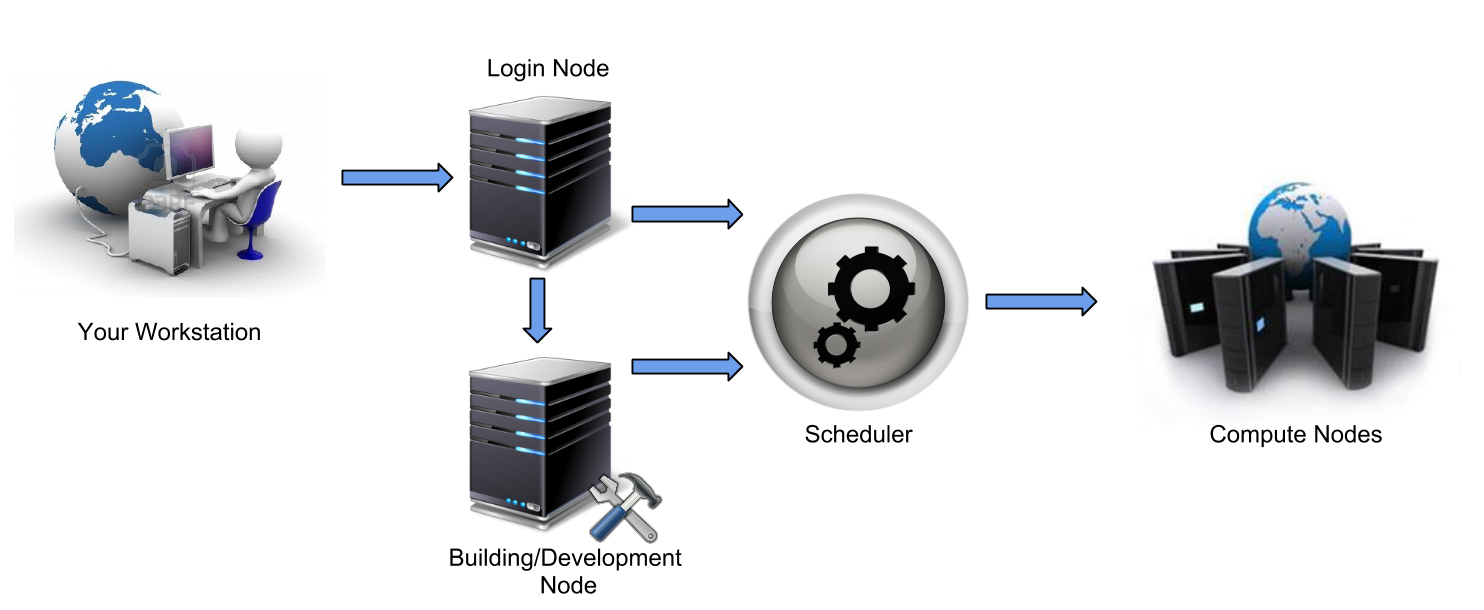
\includegraphics[width=310pt]{NeSI_img/NeSI_compute_path.png}
\end{center}
  \end{block}
}

\subsection{Suitable Work}
\frame[t]
{
  \frametitle{What to Expect}
      \begin{block}{Suitable Work}
   \begin{itemize}%[<+-| alert@+>]
	\item Problems that can be solved with parallel processing.
	\item Problems that consume large amounts of memory.
	\item Problems that render your desktop useless for long periods of time.
   \end{itemize}
  \end{block}
        \begin{block}{Less suited}
   \begin{itemize}%[<+-| alert@+>]
	\item Windows only software.
	\item Interactive software, e.g.\ GUI, only available for development. 
   \end{itemize}
  \end{block}
}

\subsection{What to expect}

\frame[t]
{
  \frametitle{What to expect}
      \begin{block}{Suitable Work}
   \begin{itemize}%[<+-| alert@+>]
	\item Some problems are ``embarrassingly parallel'' i.e.\ it is trivial to divide the problem and solve independently.\\e.g. run simulation with 1000 different initial conditions
	\item Approximately linear speedup
	\item Other problems have dependencies, they cannot be separated\\e.g. simulate the weather
	\item Speed up depends what \% of the program runtime can be parallelised
   \end{itemize}
  \end{block}
}

\subsection{Parallel speedup}

\frame[t]
{
\begin{topcolumns}
\column{0.5\textwidth}
    \begin{block}{Amdahl’s Law}
    \begin{center}
      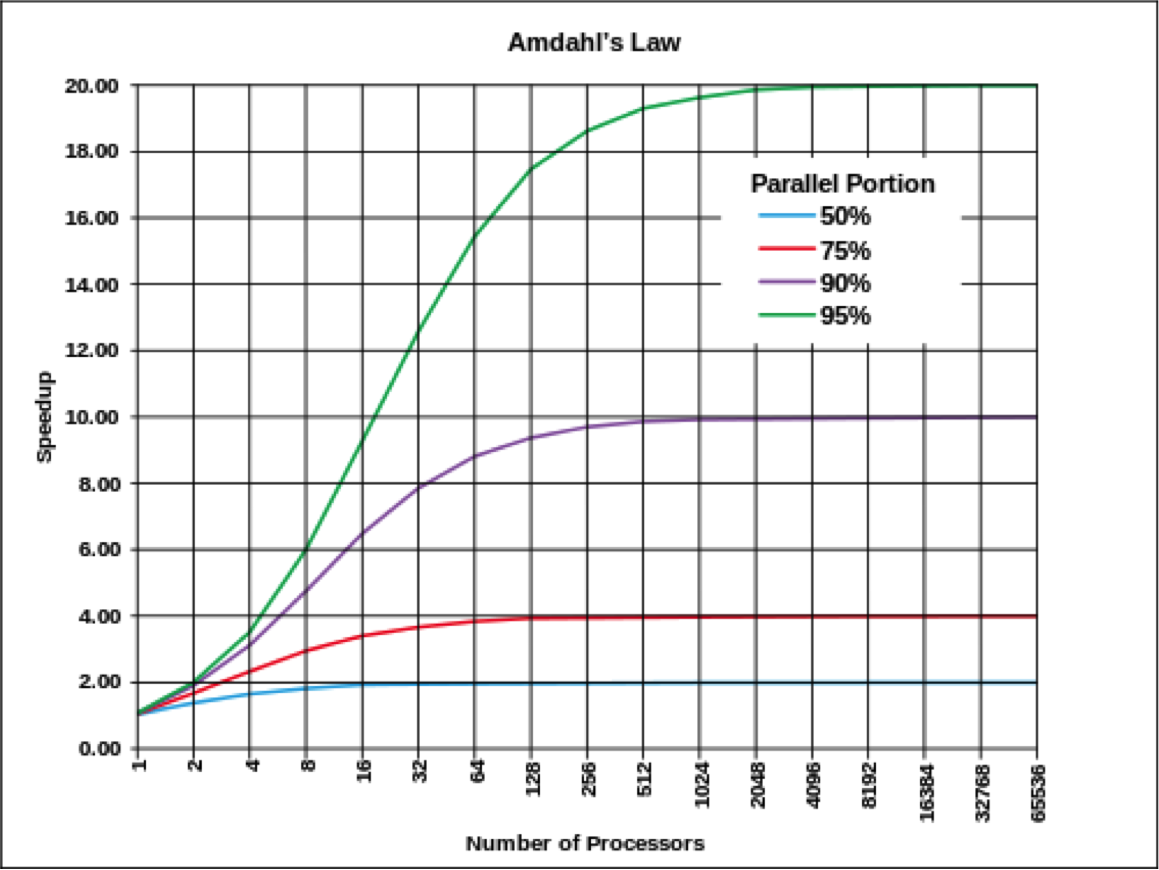
\includegraphics[width=120pt]{NeSI_img/Amdahl.png}
    \end{center}
    \end{block}
\column{0.5\textwidth}
     \begin{block}{Real Case: more cores $\neq$ more speed}
   \begin{center}
   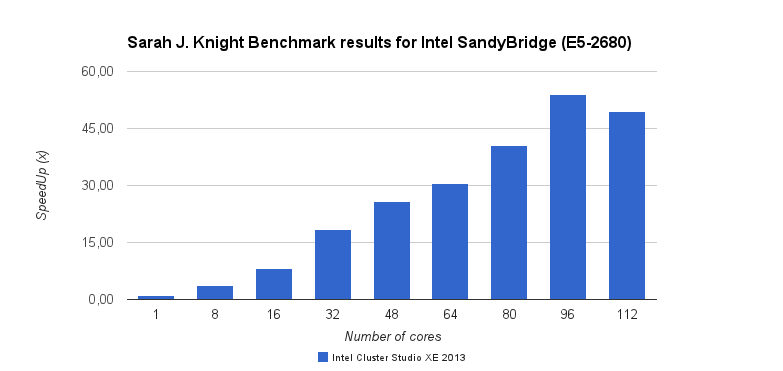
\includegraphics[width=160pt]{NeSI_img/migrate_scalability.png}
   \end{center}
  \end{block}
  \end{topcolumns}
}

\frame[t]
{
   \begin{block}{Parallel execution time}
   \begin{itemize}%[<+-| alert@+>]
	\item Single core computation time: computation only.
	\item Parallel computation time: computation + communication + waiting.
	\item E.g.\ writing results (to one file) is often a bottleneck.
	\item Small problem on many cores: communication cost will dominate.
	\item Unbalanced load: one core will mainly wait on the other.
	\item Conclusion: Test which number of cores is best suited for your problem. 
   \end{itemize}
  \end{block}
     \begin{block}{Conclusion}
   \begin{itemize}%[<+-| alert@+>]
	\item Test which number of cores is best suited for your problem. 
   \end{itemize}
  \end{block}
}


\subsection{Data}
\frame[t]
{
  \frametitle{Using the Cluster}
      \begin{block}{Data}
   \begin{itemize}%[<+-| alert@+>]
	\item Upload input data to the login node for use on the cluster.
	\item Download results from the login node to your local drive. 
	\item The home directory has a rather small quota, project directories can be larger.
	\item For long term storage and back-up, ask your IT department.
	\item Things do go wrong, make sure to have a back-up.
	\item Files on the login node are shared across the build and compute nodes
   \end{itemize}
%   \begin{center}
%   
\includegraphics[width=125pt]{NeSI_img/kami23-doubtux.png}
%   \end{center}
  \end{block}
}


\subsection{Getting to the Login Node}
\frame[t]
{
  \frametitle{Using the Cluster}
      \begin{block}{Connection via SSH}
      Each terminal client has its own way of using the Secure Shell (SSH) protocol
        \begin{itemize}
        \item Windows: \href{http://mobaxterm.mobatek.net/}{mobaxterm}
        \item MacOSX: Terminal(Included in the OS), \href{http://www.iterm2.com/}{iTerm2}
        \item Linux: \href{http://konsole.kde.org/}{Konsole}, GnomeTerminal, \href{http://yakuake.kde.org/}{yakuake}
        \end{itemize}
        On Unix based systems you need to do something like:\\ssh \url{jbon007@login.nesi.org.nz}
      \end{block}
}


\frame[t]
{
  \frametitle{Using the Cluster}
  \begin{block}{Each NeSI Supercomputing Center has one or more Login Nodes}
   \begin{itemize}%[<+-| alert@+>]
	\item \textbf{Bluefern}
	   \begin{itemize}%[<+-| alert@+>]
	    \item \url{kerr.canterbury.ac.nz} which is the AIX unix login node.
	    \item {\url{beatrice.canterbury.ac.nz}} which is the SUSE linux login node.
	    \item {\url{foster.canterbury.ac.nz}} which is the BlueGene/P login node
	    \item {\url{popper.canterbury.ac.nz}} which is the Visualization Cluster login node.
   \end{itemize}
   	\item \textbf{NIWA}
	   \begin{itemize}%[<+-| alert@+>]
	    \item {\url{fitzroy.nesi.org.nz}} which is the AIX unix login node.
      \end{itemize}
	\item \textbf{CeR}
	   \begin{itemize}%[<+-| alert@+>]
	    \item {\url{login.uoa.nesi.org.nz}} which is the RHEL linux login node.
	    %\item visual.uoa.nesi.org.nz  which is the Visualization Cluster login node.
       \end{itemize}
   \end{itemize}
  \end{block}
}


\begin{frame}[fragile]
  \frametitle{Using the Cluster}
      \begin{block}{Remote File System Access}
       In order to access the file system (/home) remotely from your machine, we recommend:
        \begin{itemize}
        \item \textbf{Windows} (mobaxterm) : \href{http://mobaxterm.mobatek.net/}{mobaxterm}
        \item \textbf{Windows} (SSHFS) : \url{http://code.google.com/p/win-sshfs/}
        \item \textbf{MacOSX} (SSHFS) : \url{http://code.google.com/p/macfuse/}
        \item \textbf{Linux} (SSHFS) : \url{http://fuse.sourceforge.net/sshfs.html}
        \item \textbf{KDE} (Konqueror) : type fish://user@host:port
        \item \textbf{Gnome} (Nautilus) : type sftp://user@host:port
      \end{itemize}
      \end{block}
\end{frame}

%\begin{frame}[fragile]
%  \frametitle{Using the Cluster}
%      \begin{block}{Remote File System Transfer with RSYNC (Unix Only)}
%       \textbf{RSYNC} over SSH protocol is the best choice to transfer big data.
%        \begin{itemize}
%        \item Transfer data from your machine to the server:\\ {\small \verb|rsync -avHl  /path/origin/* sshserver:/path/destination/|}
%        \item Transfer data from the server to your machine:\\ {\small \verb|rsync -avHl  sshserver:/path/destination/* /path/origin/|}
%        \end{itemize}
%      \end{block}
%      \begin{block}{Remote File System Transfer with scp/sftp (Unix Only)}
%       \textbf{SCP} and \textbf{SFTP} are the most popular software to transfer data across SSH protocol.
%        \begin{itemize}
%        \item {\small \verb|scp -pr sshserver:/path/origin/* path/destination/|}
%        \item {\small \verb|sftp sshserver:/path/origin/* path/destination/|}
%        \end{itemize}
%      \end{block}      
%\end{frame}



\section{Submitting a Job}
\subsection{Documentation}
\frame[t]
{
  \frametitle{Submitting a Job}
      \begin{block}{Documentation}
   \begin{itemize}%[<+-| alert@+>]
	\item Center specific documentation:
	\begin{itemize}
	\item Bluefern : \url{http://wiki.canterbury.ac.nz/display/BlueFern}
	\item NIWA : \url{http://teamwork.niwa.co.nz/display/HPCF/NIWA+HPCF+User+Documentation}
	\item CeR : \url{http://wiki.auckland.ac.nz/display/CERES/}
	\end{itemize}
	\item Examples for submitting jobs are on our Wiki page 
	\item See the ''Getting Started section''
	\item Take a look to the Quick Reference Guide. \url{http://goo.gl/ytbRWy}
	\item You will also find links to available software on the cluster
   \end{itemize}
  \end{block}
}

\subsection{Basic Job Properties}
\frame[t]
{
  \frametitle{Submitting a Job}
      \begin{block}{Basic Job Properties}
   \begin{itemize}%[<+-| alert@+>]
	\item \textbf{Name} So you can identify the output later.
	\item \textbf{Job Type} How many processes and how many threads?
	%\item \textbf{Command} What command to execute on the cluster e.g "echo hello"
	\item \textbf{Walltime} How long the job can run for. The job will be cancelled if the walltime is exceeded. 
	\item \textbf{Memory} How much memory to use? Job will die if memory is exceeded.
	\item \textbf{CPU cores} How many to use? Your program may try to use more than you request e.g.\ MATLAB.
	%\item \textbf{Files} You need to specify where additional files can be found and change references in your scripts
	\item \textbf{Account or Group information} Especially important for access to licensed software and funded research allocations
	\item \textbf{Emails} Notification of job starting, also scheduler errors.
   \end{itemize}
  \end{block}
}


\frame[t]
{
  \frametitle{Submitting a Job}
   \begin{block}{Two main tools for submitting a job}
   \begin{itemize}%[<+-| alert@+>]
	\item LoadLeveler – for people comfortable with the Linux command line
	\item Grisu Template Client – for a graphical interface
   \end{itemize}
  \end{block}
   \begin{block}{Which one to use? In general}
   \begin{itemize}%[<+-| alert@+>]
	\item LL for complex workflows or large numbers of jobs
	\item Grisu for simple workflows or few jobs 
   \end{itemize}
  \end{block}
}



\subsection{Outputs}
\frame[t]
{
  \frametitle{Submitting a Job}
      \begin{block}{Outputs}
   \begin{center}
   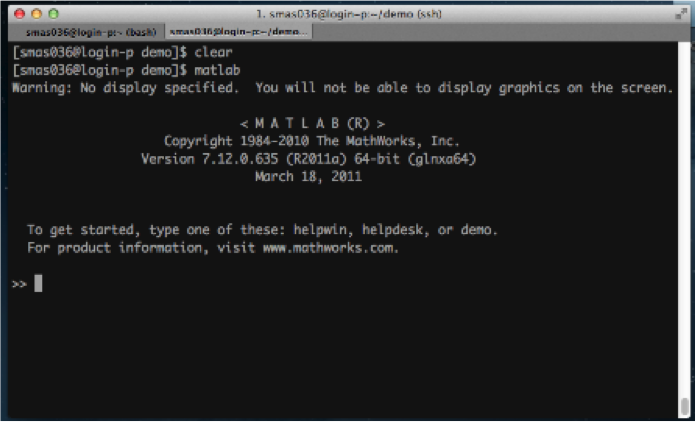
\includegraphics[width=200pt]{NeSI_img/console.png}\\
      Jobs have no interactive interface, but command line output and can write to files. Graphical tools are, however, available on the login and build/development nodes.
   \end{center}      
  \end{block}
}


\frame[t]
{
  \frametitle{Submitting a Job}
      \begin{block}{Outputs}
   \begin{itemize}%[<+-| alert@+>]
	\item Information output while the job runs is written to a text file.
	\item Standard output goes to stdout, standard error goes to stderr.
	\item These should have unique names for a given job directory (see job Name)
	\item If your application writes to other files e.g.\ output data, that stays the same
	\item When your job fails, first look at stdout and stderr for clues
   \end{itemize}
  \end{block}
}



\subsection{Grisu}
\frame[t]
{
  \frametitle{Submitting a Job}
      \begin{block}{Quick Intro to Grisu}
   \begin{itemize}%[<+-| alert@+>]
	\item Cross platform Java client: Windows, Mac, Linux
	\item Grisu interfaces with LoadLeveler to submit and monitor jobs
	\item Basic workflow:
	\item Login
	\item Set requirements
	\item Attach files
	\item Submit job
	\item Wait … check status
	\item Download results
   \end{itemize}
  \end{block}
}



\subsection{LoadLeveler}
\frame[t]
{
  \frametitle{Submitting a Job}
      \begin{block}{Quick Intro to LoadLeveler}
   \begin{itemize}%[<+-| alert@+>]
	\item You need to access the login node and work from a terminal
	\item Requires basic knowledge of the Linux command line:
   \begin{itemize}%[<+-| alert@+>]
	\item How to navigate file system and edit files
	\item Shell scripting is very useful for automation
	\item Tutorials available online at Software Carpentry – computing basics aimed at researchers
   \end{itemize}
   \end{itemize}
  \end{block}
}




\begin{frame}[fragile,shrink]
  \frametitle{Submitting a Job}
      \begin{block}{Setup a Job Description}
Can use macros in job attributes
\begin{verbatim}
e.g. #@ output = $(job_name).$(jobid).out
\end{verbatim}
MPI jobs
\begin{verbatim}
#@ job_type = MPICH | parallel
#@ total_tasks = 16
#@ blocking = 4 | unlimited
\end{verbatim}
  \end{block}

\end{frame}


\begin{frame}[fragile,shrink]
  \frametitle{Submitting a Job}
      \begin{block}{Setup a Job Description}
GPUs
\begin{verbatim}
#@ resources = … GPUDev(1)
\end{verbatim}

Specific architectures
\begin{verbatim}
#@ requirements = (Feature==“sandybridge”)
#@ requirements = (Feature==“Kepler”)
\end{verbatim}
  \end{block}
\end{frame}


\begin{frame}[fragile,shrink]
  \frametitle{Submitting a Job}
%      \begin{block}{Job Description Example : SMP}
\begin{verbatim}
#!/bin/bash 
# Optimized for run parallel job of 12 Cores in NeSI (Pandora-westmere)
##########################################################################
#@ job_name = Gaussian
#@ class = default
#@ notification = never
#@ group = nesi
#@ account_no = uoa
#@ wall_clock_limit = 1:00
#@ initialdir = $(home)
#@ output = $(home)/$(job_name).txt
#@ error = $(home)/$(job_name).err
#@ job_type = serial
#@ resources = ConsumableMemory(2048mb) ConsumableVirtualMemory(2048mb)
#@ parallel_threads = 12
#@ environment = COPY_ALL,OMP_NUM_THREADS=12
#@ queue
########################################################################## 
module load g09/C.01
cd $SCRATCH_DIR
cp -r $HOME/Gaussian/h2o_opt.dat . 
setenv GAUSS_SCRDIR $SCRATCH_DIR
###  Run the Parallel Program
g09 < ./h2o_opt.dat > h2ol_opt.log
###  Transfering the results to the home directory ($HOME) 
cp -pr $TMP_DIR $HOME/results/
\end{verbatim}
%  \end{block}
\end{frame}

\begin{frame}[fragile,shrink]
  \frametitle{Submitting a Job}
%      \begin{block}{Job Description Example : MPI}
\begin{verbatim}
#!/bin/bash
# Optimized for run parallel job of 512 Cores at NeSI (Pandora-SandyBridge)
##########################################################################
#@ job_name = LAMMPS_TEST
#@ class = default
#@ group = nesi
#@ notification = never
#@ account_no = uoa
#@ wall_clock_limit = 00:30:00
#@ resources = ConsumableMemory(4096mb) ConsumableVirtualMemory(4096mb)
#@ job_type = MPICH
#@ blocking = unlimited
#@ node_usage = not_shared
#@ output = $(job_name).$(jobid).out
#@ error = $(job_name).$(jobid).err
#@ requirements = (Feature=="sandybridge")
#@ initialdir = /share/src/LAMMPS/lammps-12Aug13/bench
#@ total_tasks = 512
#@ queue
##########################################################################
module load lammps/12Aug13-sandybridge
cd $SCRATCH_DIR
cp /share/test/LAMMPS/* .
###  Run the Parallel Program
export OMP_NUM_THREADS=1
MPIRUN lmp_mpi -var x 20 -var y 20 -var z 20 -in in.lj > lj-512.out
###  Transfering the results to the home directory ($HOME)
cp -pr $SCRATCH_DIR $HOME/OUT/lammps/
\end{verbatim}
%  \end{block}
\end{frame}

%\frame[t]
%{
%  \frametitle{Submitting a Job}
%      \begin{block}{ulimit : Only for CeR!}
%   \begin{itemize}%[<+-| alert@+>]
%	\item Constrains your memory use 
%	\item LL only schedules the memory and avoids placing other potential jobs on the same nodes
%	\item Without ulimit, your process’s memory use may grow and exhaust the machine, randomly killing other processes
%	\item Grisu does this automatically
%   \end{itemize}
%  \end{block}
%}


\frame[t]
{
  \frametitle{Submitting a Job}
      \begin{block}{Environment Modules}
   \begin{itemize}%[<+-| alert@+>]
	\item Modules are a convenient way to provide access to applications on the cluster
	\item They prepare the environment you need to run the application
	\item Commands
        \begin{itemize}
        \item  \textbf{module avail} - lists available modules
        \item  \textbf{module show module\_name} - displays full information about the module with name \textit{module\_name}.
        \item  \textbf{module load module\_name} - loads the module with name \textit{module\_name} and its dependencies. 
        \item  \textbf{module unload module\_name } - unload  the module with name \textit{module\_name} and its dependencies. 
        \item  \textbf{module list} - list all modules currently loaded.
        \end{itemize}
	\item Grisu loads a module when you select an application
   \end{itemize}
  \end{block}
}


\frame[t]
{
  \frametitle{Submitting a Job}
      \begin{block}{LoadLeveler}
   \begin{itemize}%[<+-| alert@+>]
	\item To submit a job\\llsubmit myjob.ll
	\item To monitor a job\\llq –u “myuserid”
	\item Shows job id and status – R, I, etc
	\item To cancel\\llcancel “jobid”
   \end{itemize}
  \end{block}
}

\frame[t]
{
  \frametitle{Submitting a Job}
      \begin{block}{Notes for Windows Users}
   \begin{itemize}%[<+-| alert@+>]
	\item Be careful of Windows end of line (EOL) characters, sometimes Linux will not handle them correctly
	\item Notepad++ lets you convert between Windows and Unix style line endings
	\item Even though you can avoid using the Linux command line, having a basic understanding will help you debug your jobs
   \end{itemize}
  \end{block}
}




\subsection{Software}
\frame[t]
{
  \frametitle{Submitting a Job}
      \begin{block}{Software}
   \begin{itemize}%[<+-| alert@+>]
	\item We have many specialised software packages.
	\item Best way to see what we have is by checking the wiki. %running module avail on the login node
	\item The Wiki also has a software section
	\item We can install software that you need, but …
   \begin{itemize}%[<+-| alert@+>]
	\item It must run on Linux
	\item It must run in batch mode – no user interaction
	\item You must have the required licenses
	\item You can install software in your home directory if it is really esoteric
   \end{itemize}
   \end{itemize}
  \end{block}
}

\subsection{Best practices and advice}

\frame[t]
{
  \frametitle{Submitting a Job}
   \begin{block}{Best practices and advice}
   \begin{itemize}%[<+-| alert@+>]
	\item Share with us a short test and we will study the scalability of your application.
	\item Try to be accurate  with the walltime, it will help to the LL to schedule the jobs better.
	\item Be aware that you are sharing resources with other researchers.
	\item If you need to run a test for a long time (>2h) use tLL.
	\item A wrong memory request or a wrong job description setup can potentially affect others.
	\item If we find some case like that, we may be forced to cancel the job with this behaviour and inform the owner by email.
   \end{itemize}
  \end{block}
}


%\section{Our Expectations}

\frame[t]
{
  \frametitle{Our Expectations}
      \begin{block}{Our Expectations}
   \begin{itemize}%[<+-| alert@+>]
	\item We have an acceptable use policy that follows the NeSI IT policies
	\item We conduct regular reviews of projects to	:
   \begin{itemize}%[<+-| alert@+>]
	\item see how you are going and if you could use some help
	\item collect any research outputs from your work on our facility
	\item determine how the cluster has helped your research 
	\item look at the potential for feature stories on your work
   \end{itemize}
	\item Please contact us if you have any questions
	\item Please acknowledge us in your publications
%	\item We have a blurb on the Wiki front page
   \end{itemize}
  \end{block}
}


%\frame
%{
%\begin{center}
% 
\includegraphics[width=200pt]{NeSI_img/kami23-doubtux.png}
%\end{center}
%}

%\section{}
%\frame[t]
%{
%  \frametitle{}
%      \begin{block}{}
%   \begin{itemize}%[<+-| alert@+>]
%	\item 
%	\item 
%	\item 
%	\item 
%   \end{itemize}
%  \end{block}
%}

{
\setbeamertemplate{background canvas}{
\includegraphics[height=0.99\paperheight]{NeSI_img/Slide00.png}} 
\begin{frame}[plain]
\begin{center}
{\Huge Questions \& Answers}
\end{center}
\end{frame}
}


\end{document} 
